\documentclass[letterpaper]{article}
\usepackage[bookmarks,colorlinks=true,linkcolor=blue,urlcolor=blue]{hyperref}
\usepackage{url}
\usepackage{tabularx}
\usepackage{graphicx}
\usepackage{placeins}
\usepackage{paralist}
\usepackage{makecell}
\usepackage{colortbl}
\usepackage{zi4}
\usepackage{float}
\usepackage{textcomp}
\usepackage{tocloft}
\usepackage{gensymb}
\usepackage{verbatim}
\usepackage{siunitx}
\usepackage[libertine,cmbraces]{newtxmath}
\usepackage{booktabs}
\usepackage[margin=1in,top=1in,bottom=1in]{geometry}

% table lines
\setlength{\heavyrulewidth}{0.12em}
\setlength{\lightrulewidth}{0.04em}
\newcommand{\thickhline}{\toprule[\heavyrulewidth]}
\newcommand{\thinhline}{\midrule[\lightrulewidth]}

\begin{document}

\title{Construction and Circuit Analysis: Microchip PIC12F683}
\author{Andrew D. Zonenberg}
\date{\today}
\maketitle

\begin{abstract}
This report describes an extensive analysis and reverse engineering of the Microchip PIC12F683 microcontroller.

All analysis and sample preparation was performed by the author using garage laboratory facilities and open source software for professional development, entertainment, and educational purposes only; this project was not supported or sponsored by any third party.

Sample preparation was limited to basic wet chemistry and optical microscopy, to make the project more fun and challenging and to push the limits of what could be done in a home setup. SEM/FIB, dry etch, precision polishing, industry reverse engineering software, and other advanced tools were deliberately not used, even if the author had access to them via work or friends.

This report is licensed under CC BY-ND 4.0 and the LaTeX source and images used in the report can be found
\href{https://github.com/azonenberg/pic12f683-analysis}{on GitHub}.
\end{abstract}

\pagebreak
\tableofcontents

\pagebreak
\section{Device Overview}

The subject of this report is the Microchip PIC12F683-I/MD. Multiple specimens, all from the same cut tape purchased at Digi-Key with date code 2321 and lot code 9BW, were used during the analysis.

The PIC12F683 is an 8-bit microcontroller from Microchip Technology, originally developed in 2004\footnote{Based on the revision date of the oldest available documentation on Microchip's website} and still in production. It is a strict Harvard architecture with no access to flash from the data bus and no ability to execute code from RAM. The CPU is a microcoded sequential design with a maximum frequency of 20 MHz, which executes at 4 clocks per instruction for all operations other than branches which take longer. Function calls use a hardware stack with a maximum depth of eight nested calls.

It has 2048 14-bit instruction words of flash, 128 bytes of SRAM, and 256 bytes of EEPROM. The EEPROM is indirectly accessible via address/data/control registers; EEPROM data is not directly memory mapped.

It is available in four packages, all with eight pins (one power, one ground, and six I/Os): DIP (ordering code P), 3.9mm SOIC (SN), 4x4mm DFN (MD), and 6x5mm DFN (MF). Pin numbering between the packages is identical.

\pagebreak
\section{Package Analysis}

The PIC12F683 is available in multiple packages; the subject of this report used the ``MD" package which is an 8-pin saw-singulated DFN with nominal dimensions of 4 x 4 x 0.9 mm.

\subsection{PCN Search}

A search of vendor PCNs was conducted, which suggested that numerous assembly sites (designated MP3A, MTAI, NSEB, GTK, LPI, UNIS, and MMT) were used to produce this part and it was not possible to identify with certainty which one was used for the samples under test without access to internal Microchip lot traceability information or supplier databases.

A new PFAS-free die attach material ``QMI519" was qualified in September 2025\footnote{\href{https://www.microchip.com/PCNWebAPI/api/pcn/DownloadPcnDocument?pcnid=24234&fileName=PFAS\%20Elimination\%20and\%20Die\%20Attach_Explanation.pdf}{PCN CENO-16EGCZ399}} however the samples used for this analysis had 2023 week 21 date codes and thus presumably were using the older, PFAS-containing, die attach. One PCNs mentioned CRM1076DJ die attach and G770HCD mold compound\footnote{\href{https://www.microchip.com/PCNWebAPI/api/pcn/DownloadPcnDocument?pcnId=252&affectedcpns=pdf}{PCN CYER-19MGTD414}} for the 4x4 DFN; another mentioned 8600 die attach and G700LTD mold compound\footnote{\href{https://www.microchip.com/PCNWebAPI/api/pcn/DownloadPcnDocument?pcnid=6667&fileName=PCN_JAON-04FCXY806_Qual\%20Report.pdf}{PCN JAON-04FCXY806}} so any of these are likely candidates. The author's lab capabilities were not sufficient to determine with certainty which was used. Based on these and other PCNs the bond wire material was likely to be palladium coated copper and may or may not have a gold flash over the palladium plating, depending on which assembly site was used\footnote{In the author's experience, older generation PIC12F683s used gold ball bonding. The samples analyzed in this report were copper bonded and PCNs reference both CuPd and CuPdAu bond wire. Without access to SEM+EDS capabilities, it was not possible to detect the presence of the gold flash layer.}.

\subsection{Package Overview}

One sample was photographed at low magnification using a combination of through-objective and
low-angle illumination to best highlight the various materials in the package with vastly different albedos

The top side of the package (Fig. \ref{pkgtop}) was laser marked ``12F683 I/MD (e3) 2321 9BW" plus a pin 1 marker and had no other noteworthy features.

The bottom side of the package (Fig. \ref{pkgbot}) had eight tin-plated copper solder lands plus a die attach/thermal paddle with a mitered corner to denote the pin 1 position. A small amount of deformation was noted at the outboard edges of the lands, consistent with smearing of the relatively soft copper alloy by the dicing saw during the singulation process. Witness marks (Fig. \ref{probe-witness}, \ref{probe-witness2}) consistent with impressions of probe/socket contacts during factory test, could be seen on each terminal. The witness marks consisted of two circular dots approximately 37 \unit{\micro\meter} in diameter and varied slightly in spacing, suggesting that they were the result of multiple contact events with a single contact per pin (or a socket with two individual contacts per pin) rather than a single forked contact.

\begin{figure}[h]
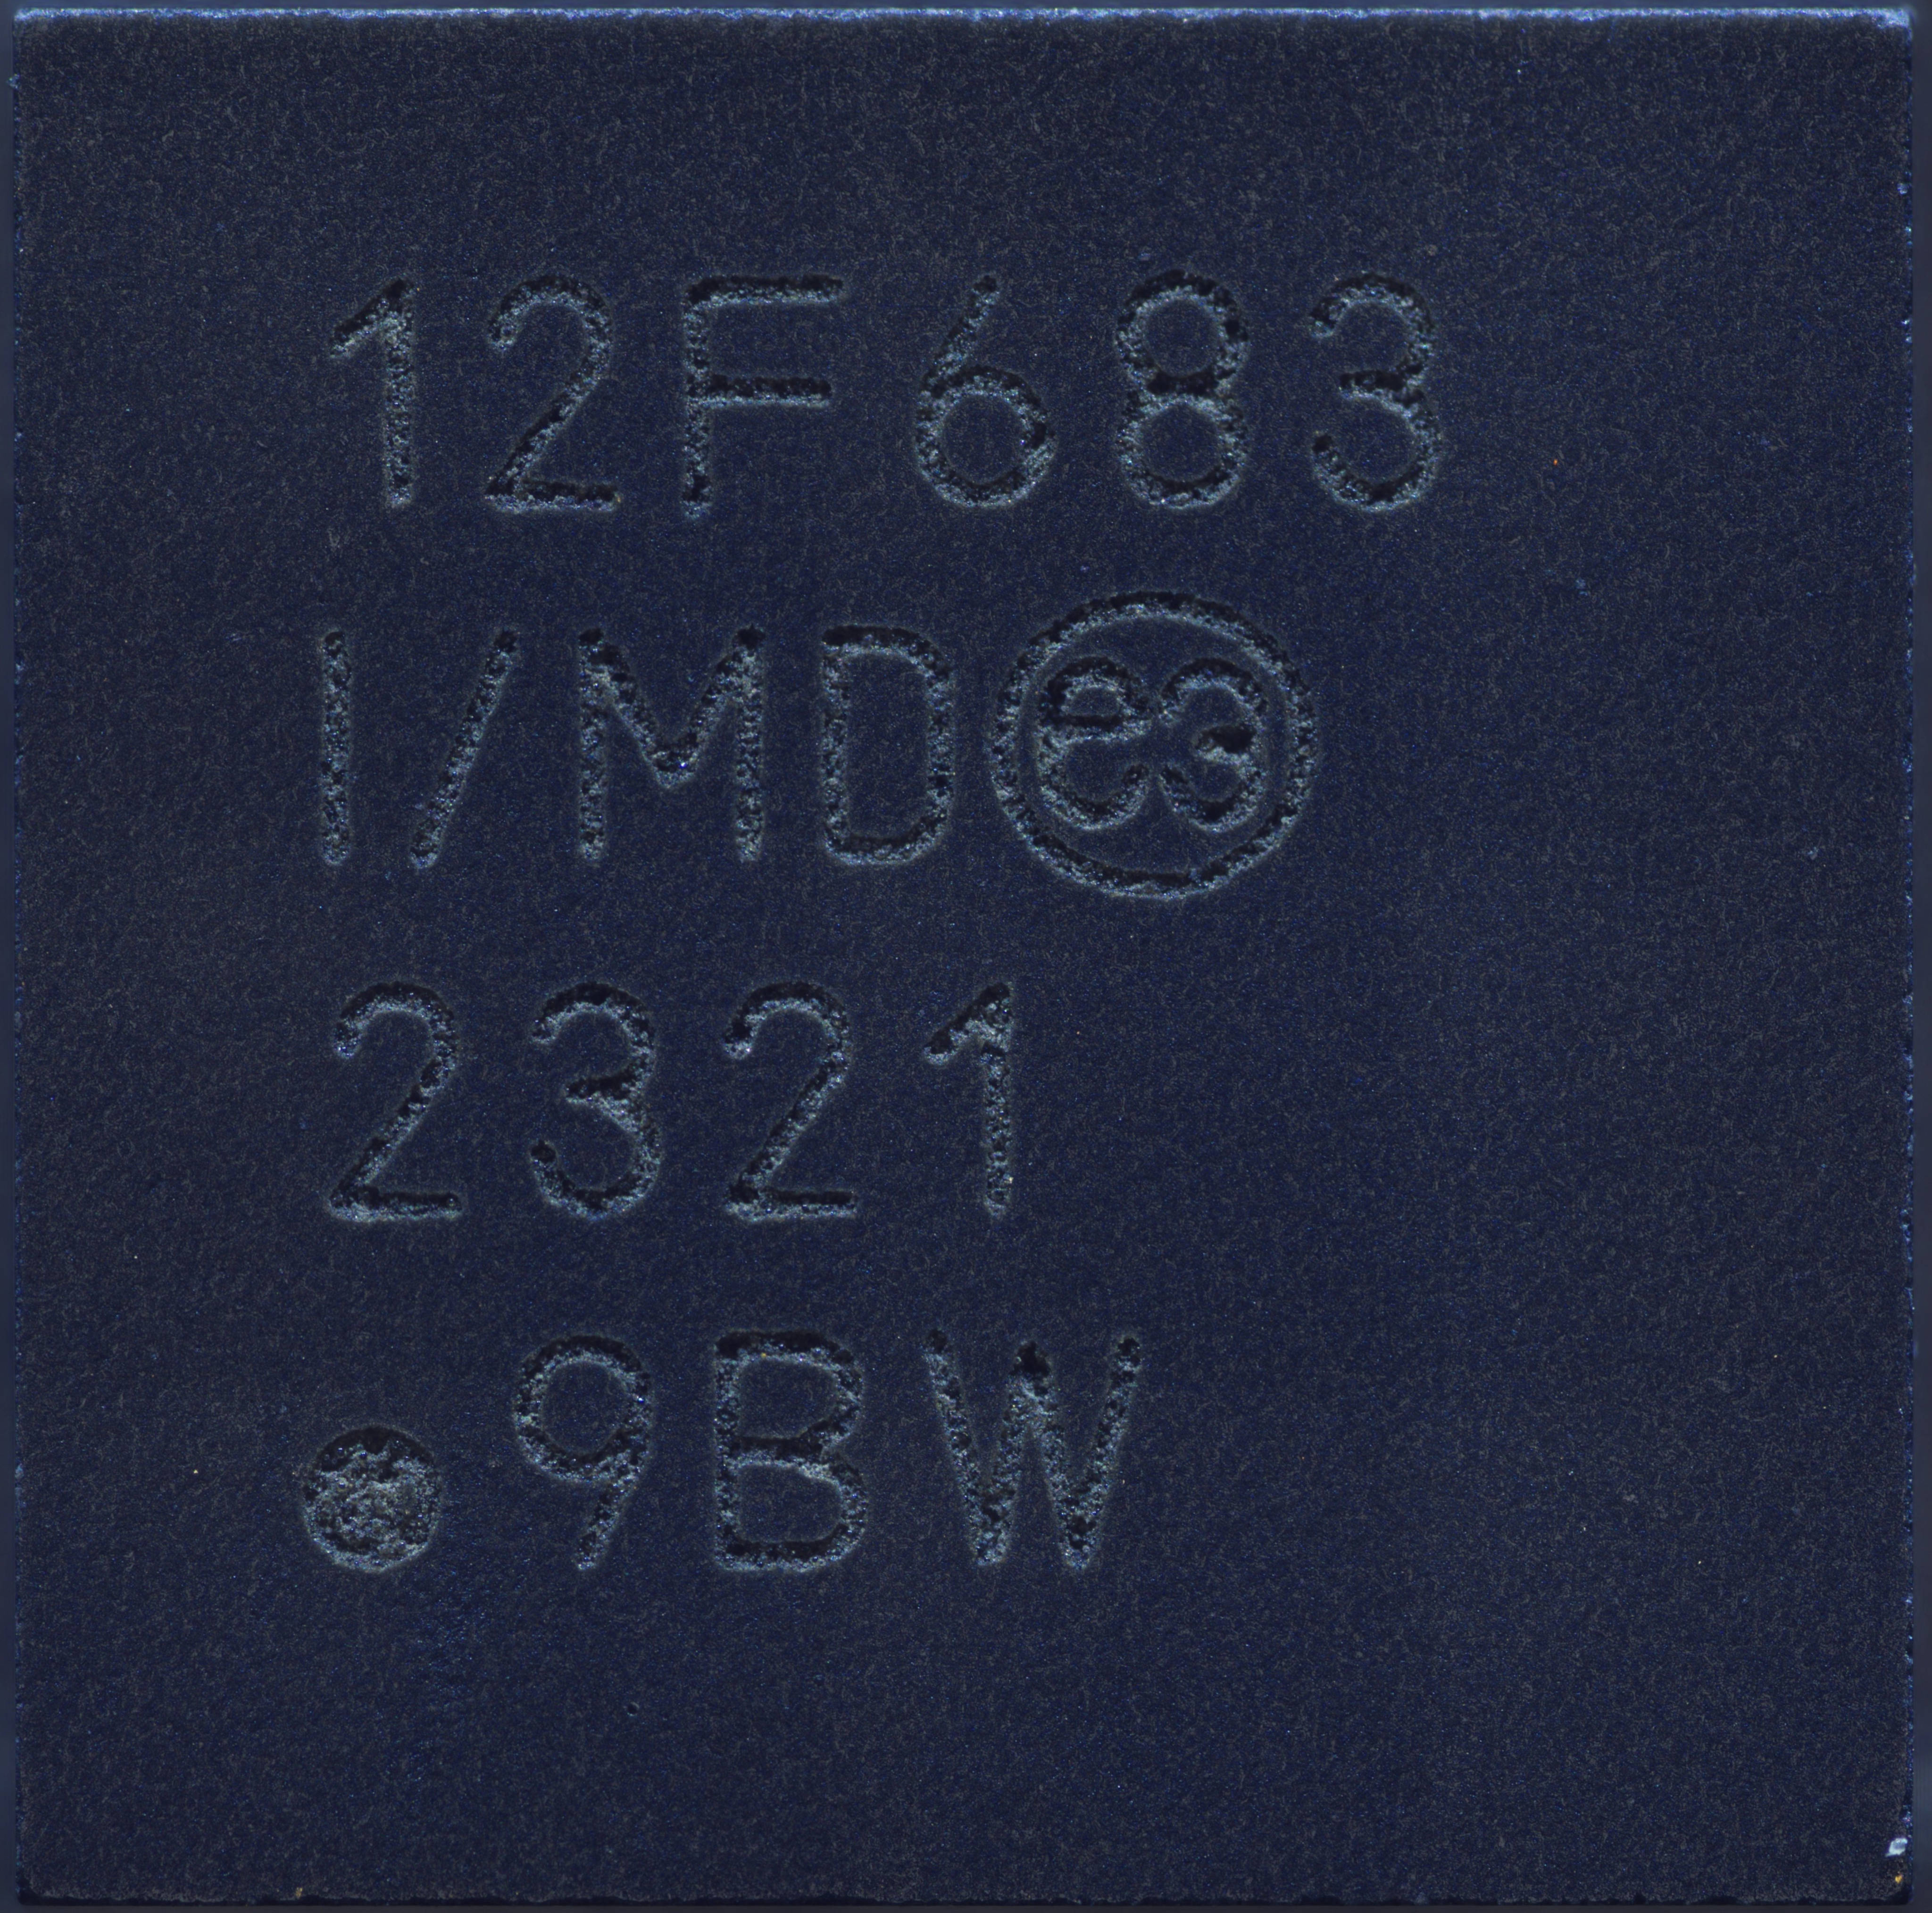
\includegraphics[width=10cm,keepaspectratio]{images/pkgtop.jpg}
\caption{Top view of package. Pin 1 in southwest corner. Mitutoyo 5x/0.14 objective.}
\label{pkgtop}
\end{figure}

\begin{figure}[h]
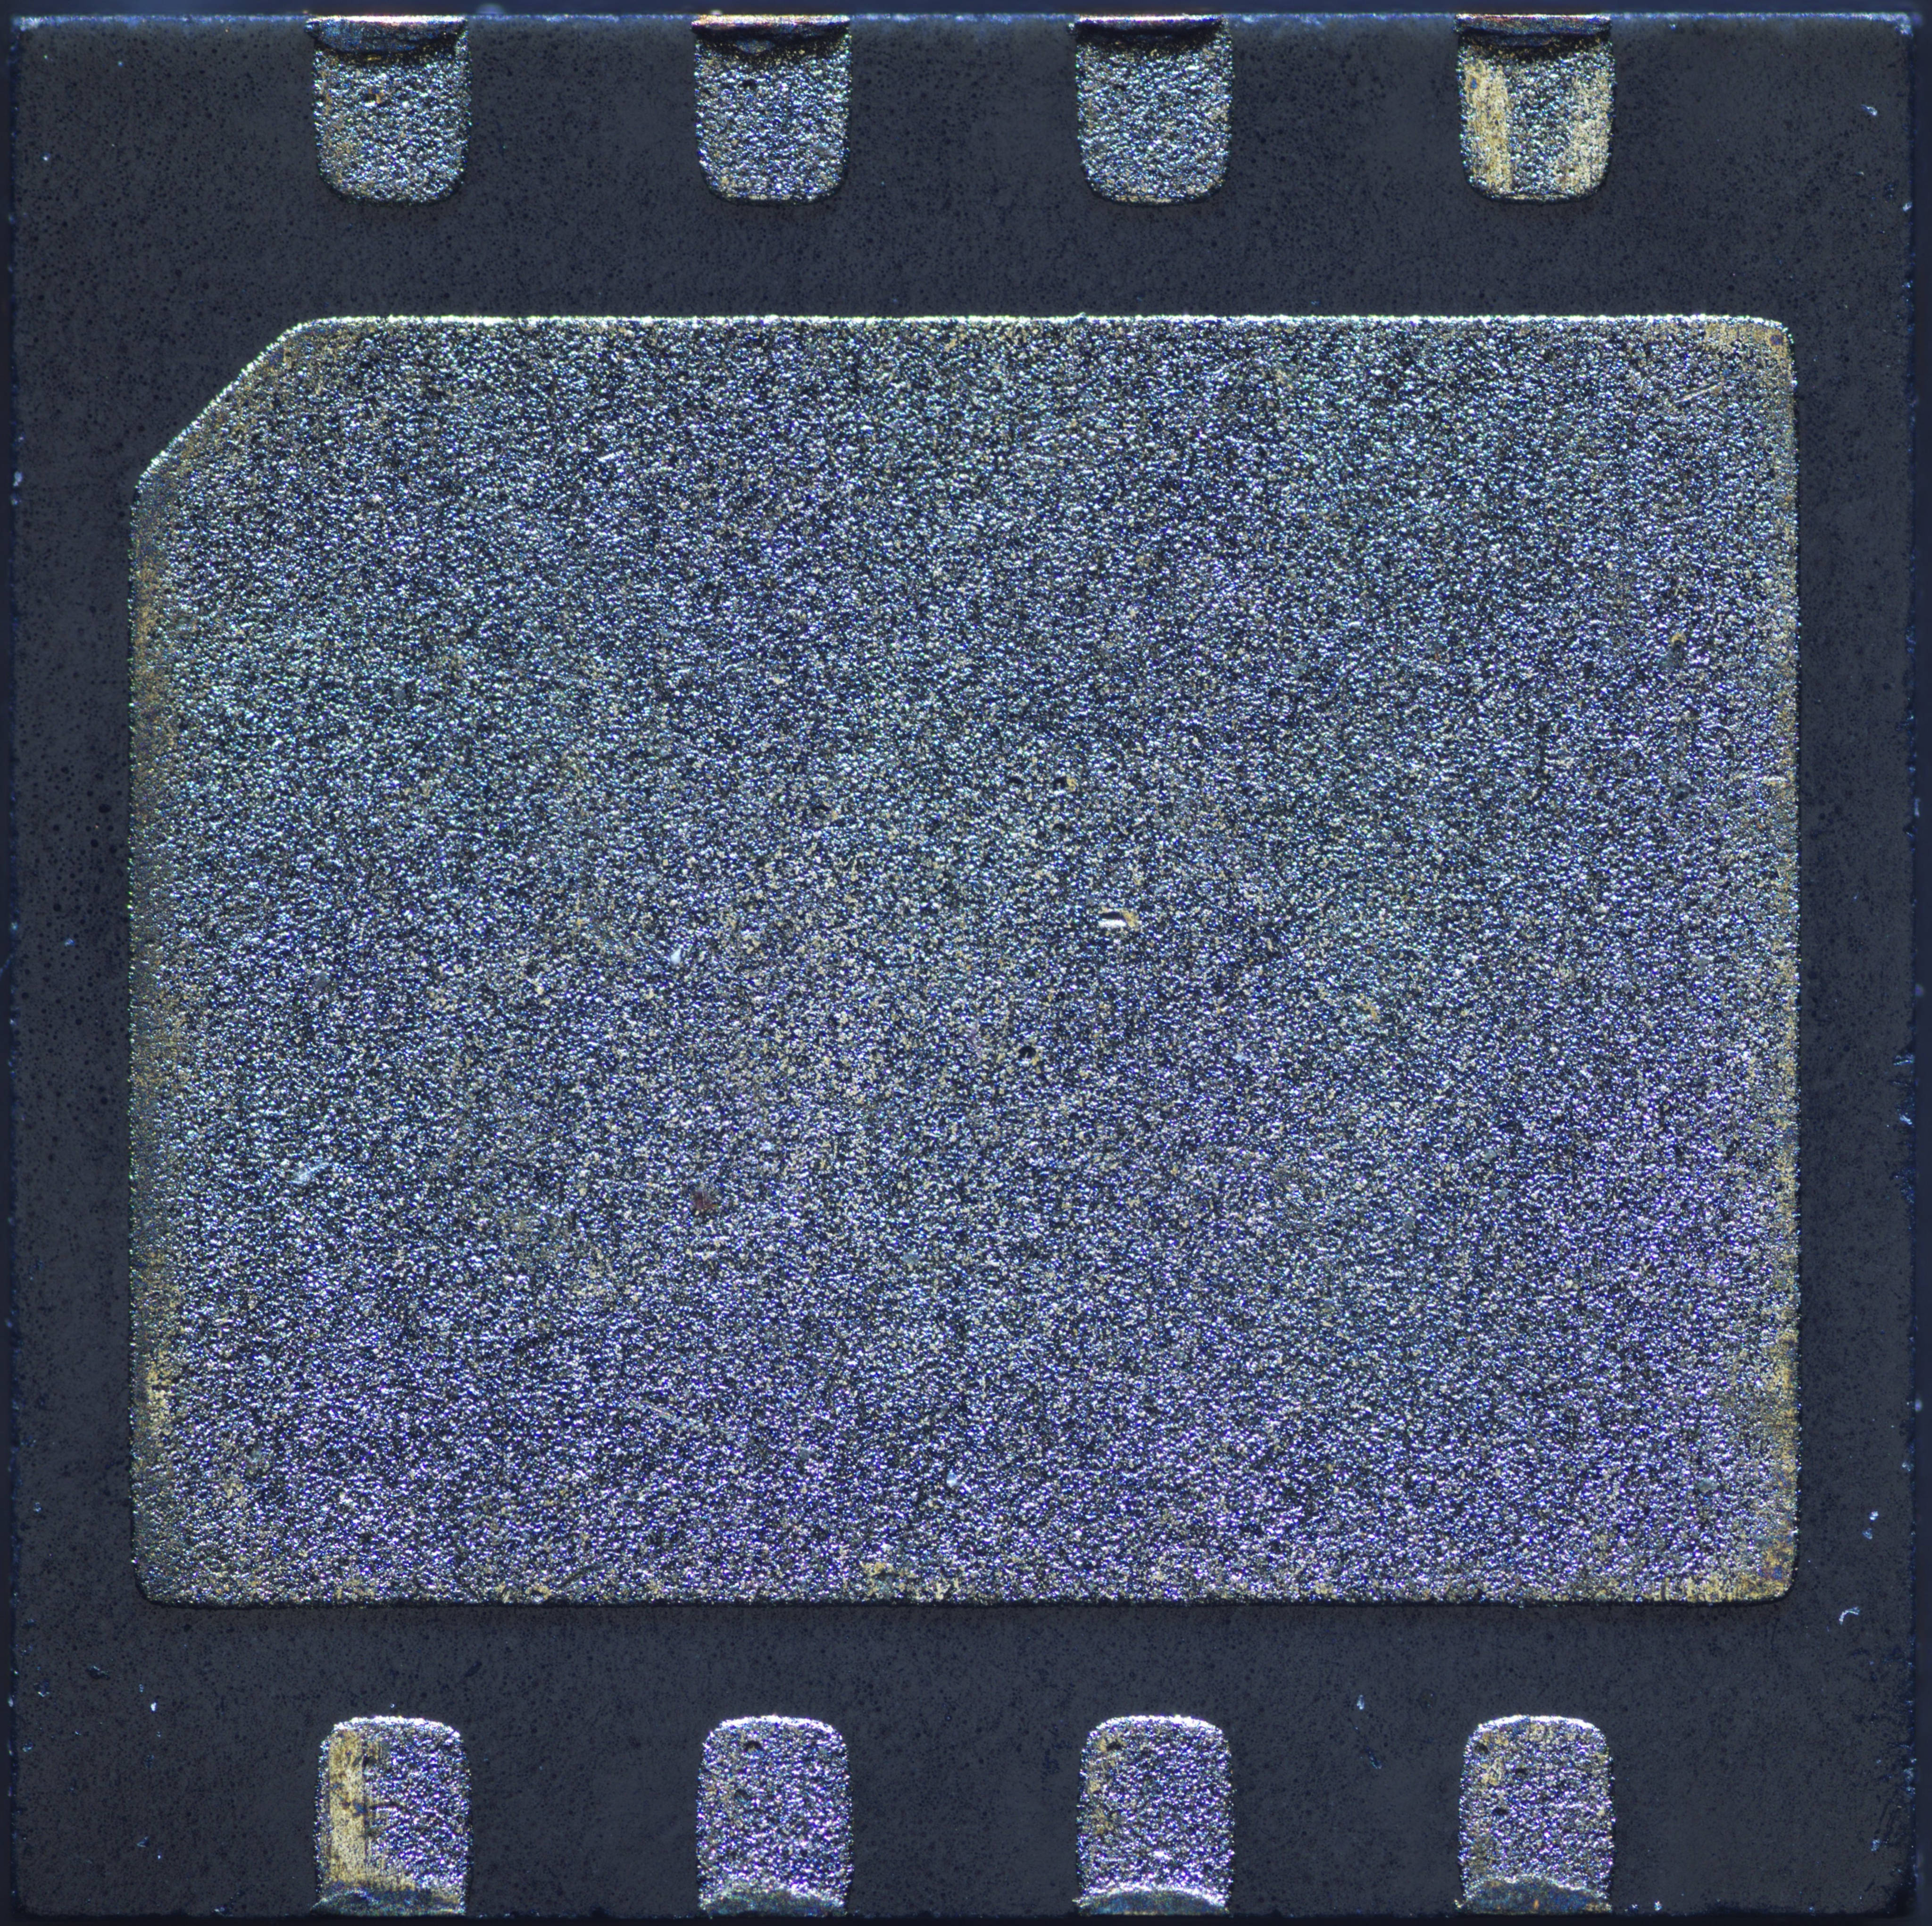
\includegraphics[width=10cm,keepaspectratio]{images/pkgbot.jpg}
\caption{Bottom view of package. Pin 1 in northwest corner. Mitutoyo 5x/0.14 objective.}
\label{pkgbot}
\end{figure}

\begin{figure}[h]
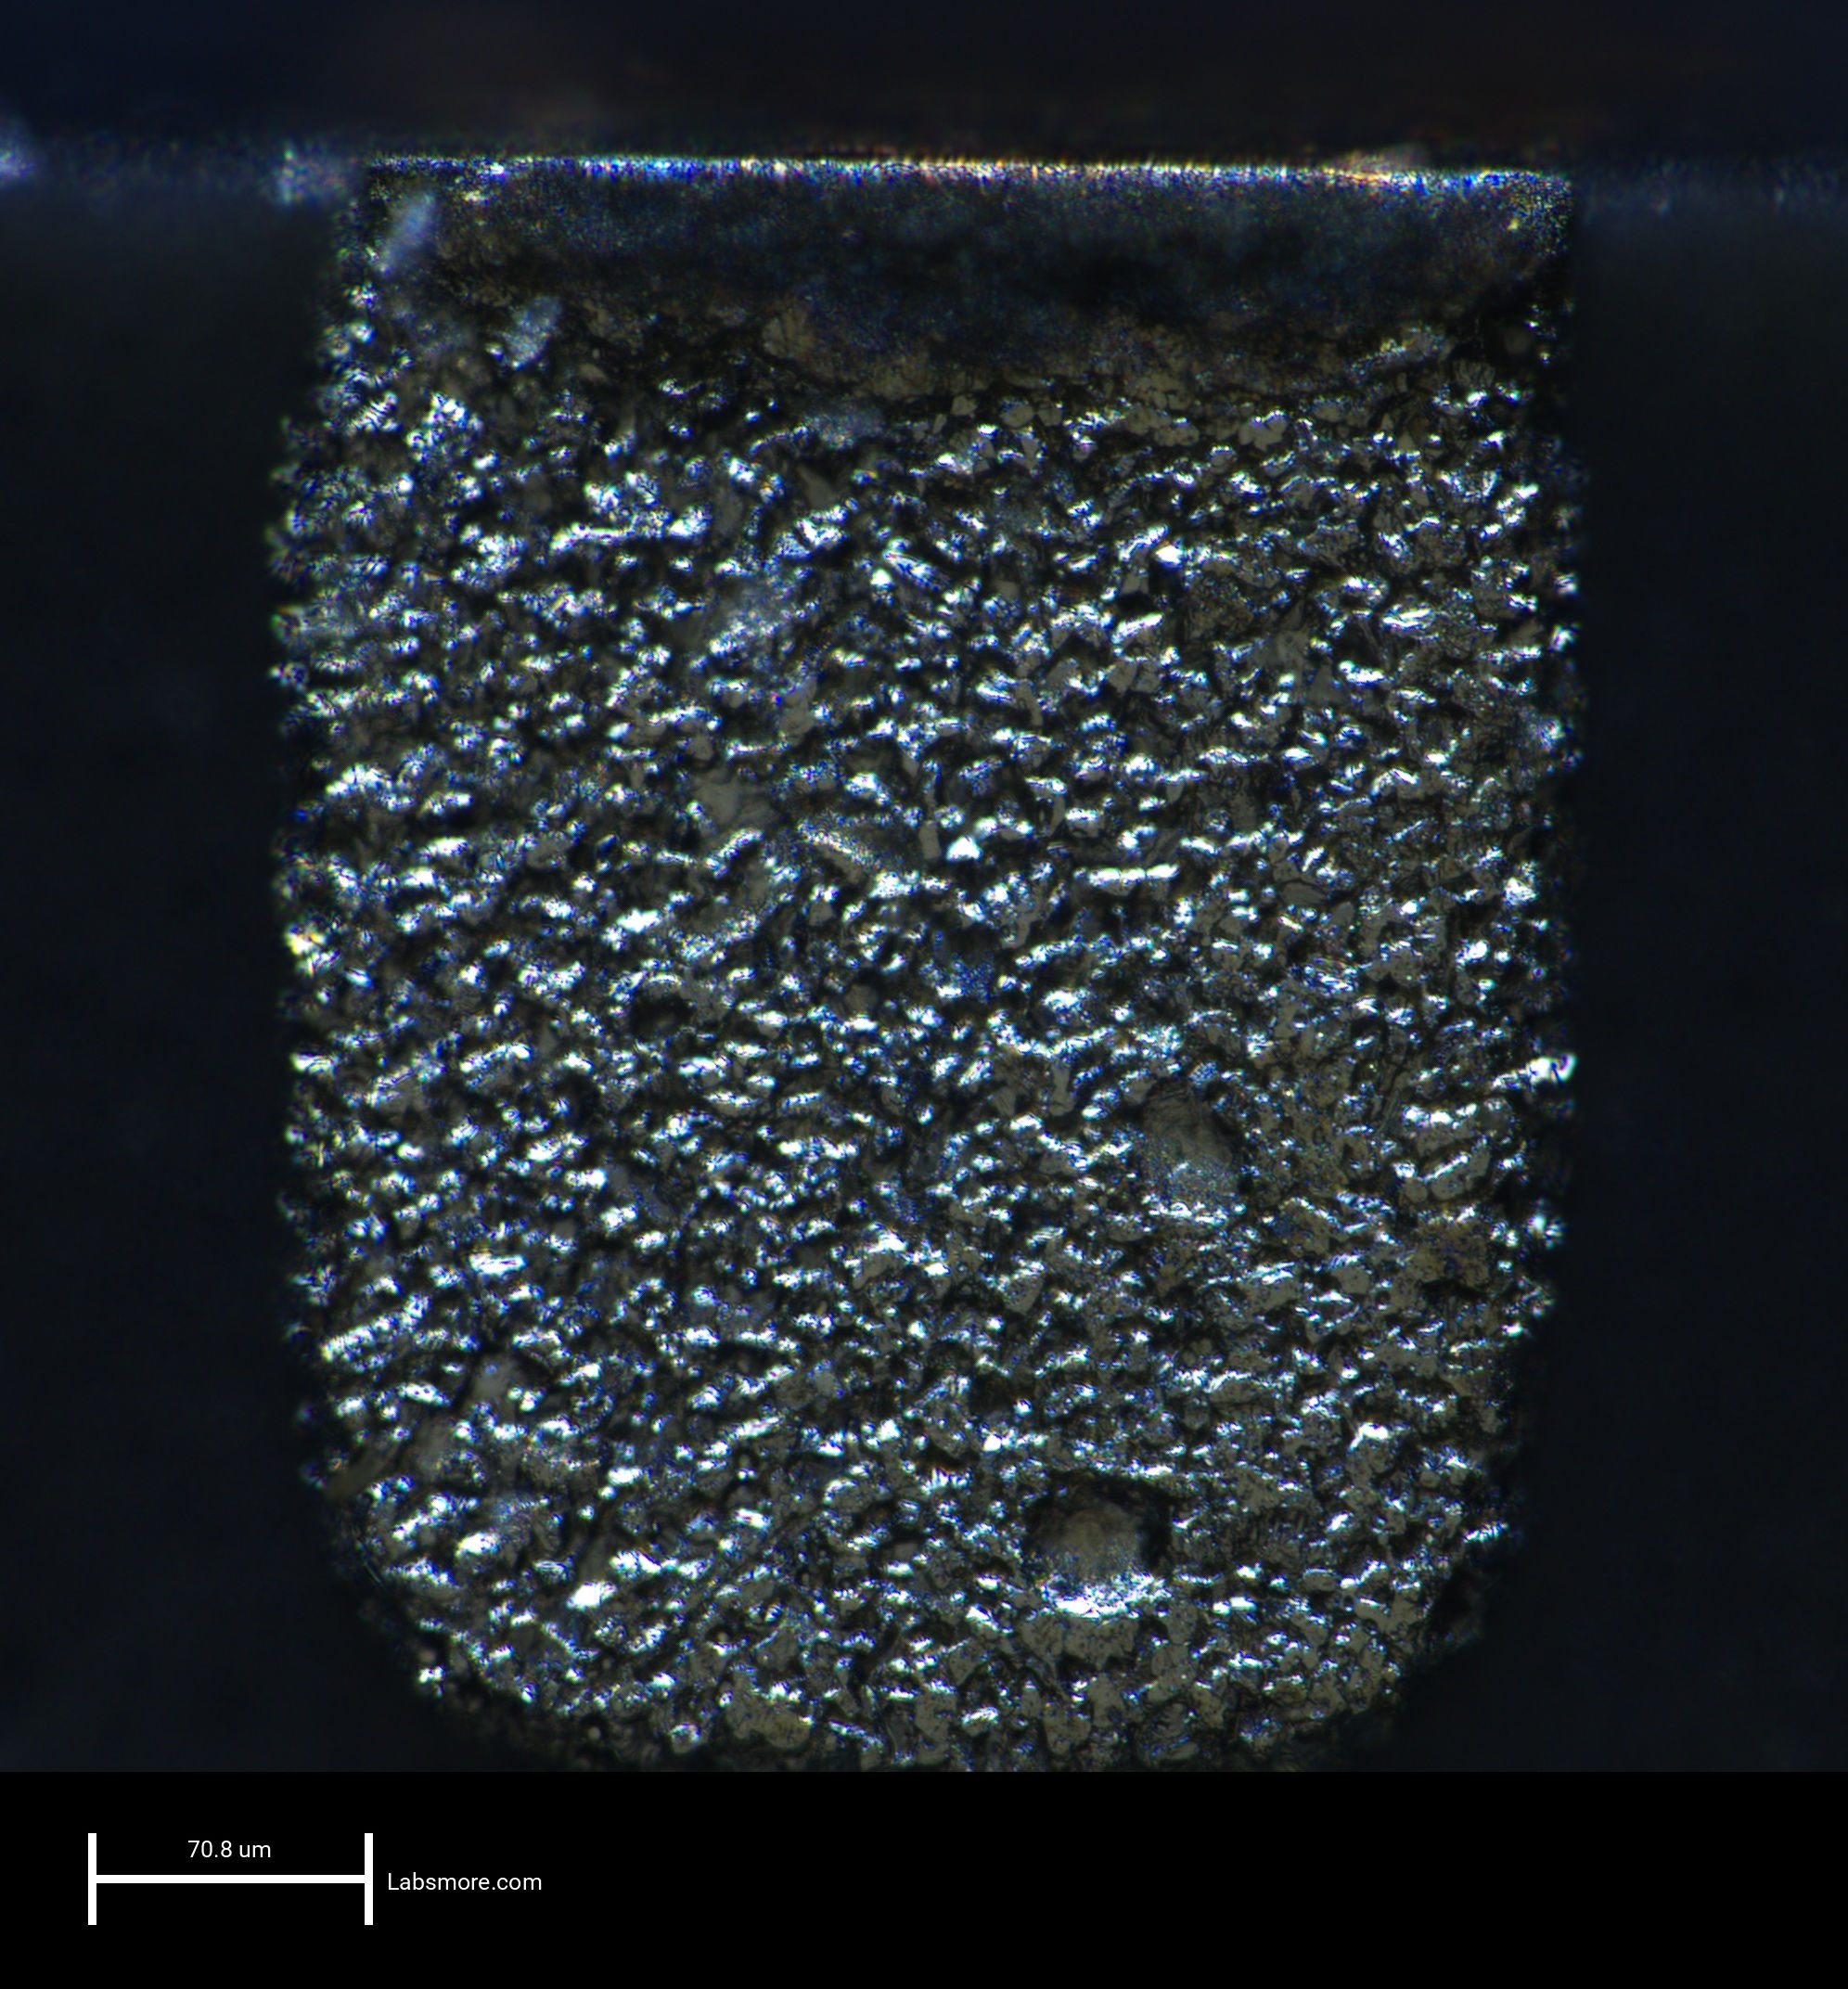
\includegraphics[width=10cm,keepaspectratio]{images/probe-witness.jpg}
\caption{Witness marks on one of the solder terminals. Mitutoyo 20x/0.42 objective.}
\label{probe-witness}
\end{figure}

\begin{figure}[h]
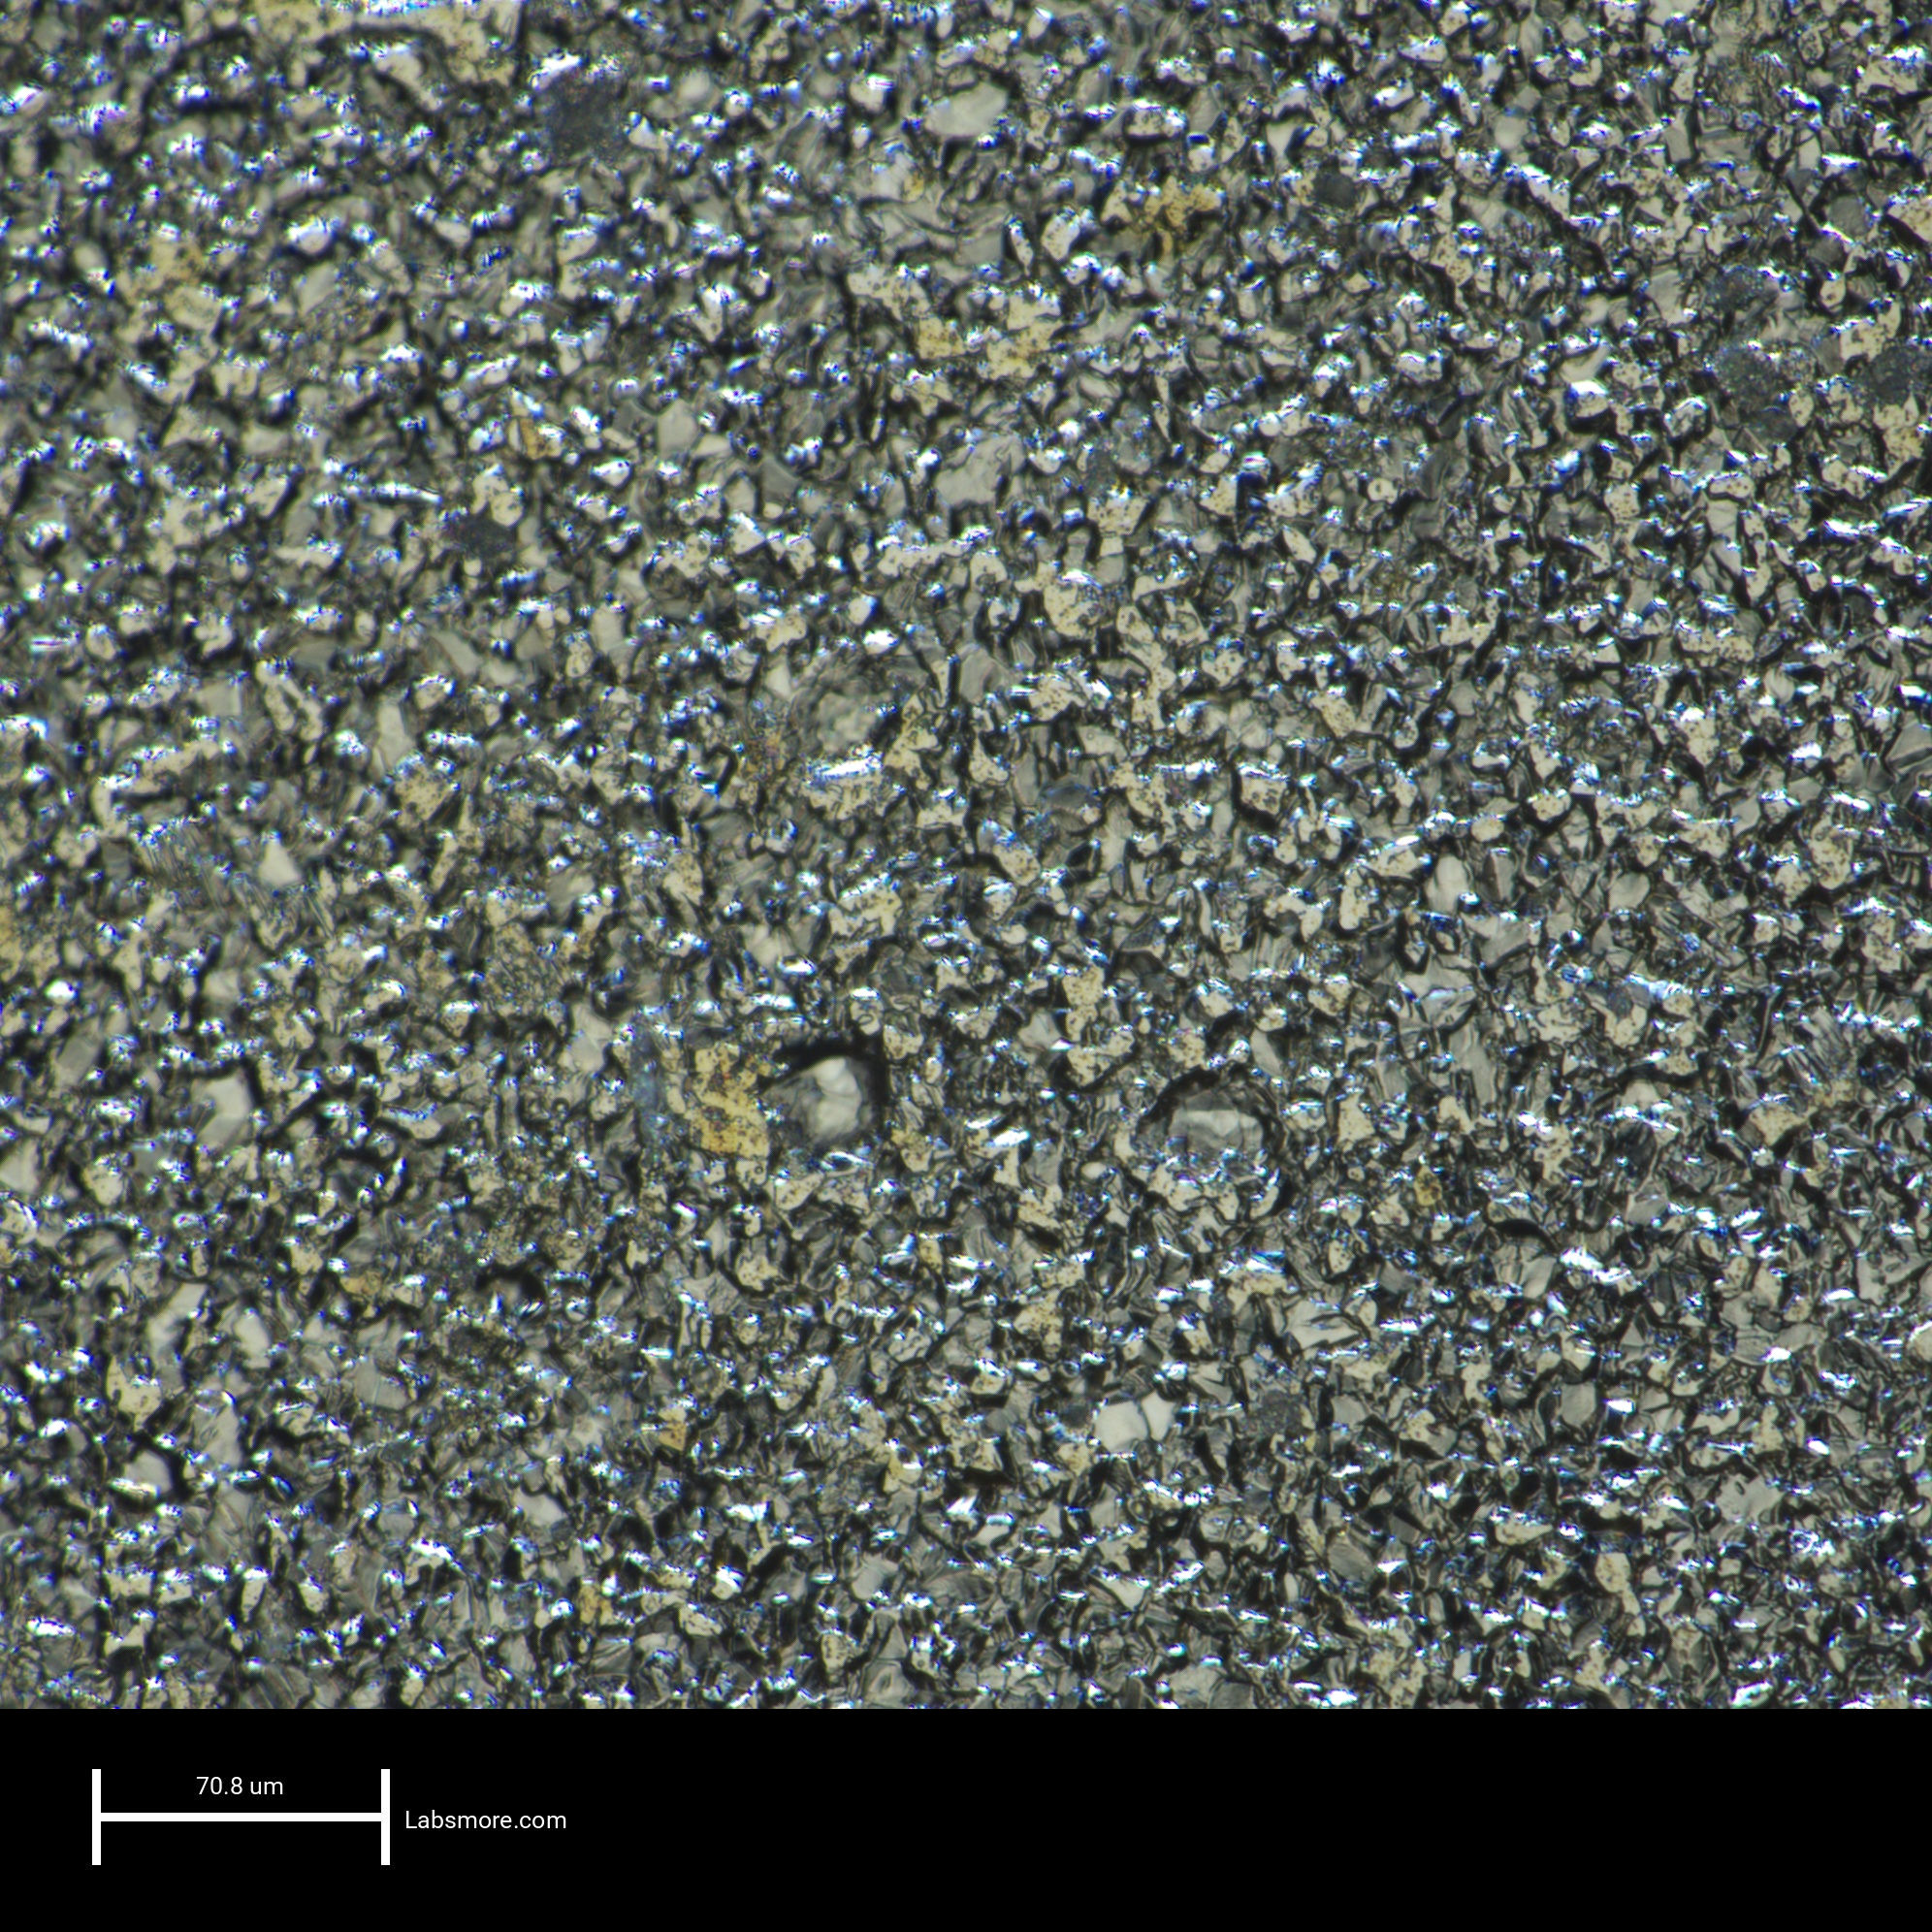
\includegraphics[width=10cm,keepaspectratio]{images/probe-witness2.jpg}
\caption{Witness marks on the center pad. Mitutoyo 20x/0.42 objective.}
\label{probe-witness2}
\end{figure}

\FloatBarrier
\subsection{Cross Section}

One sample was placed in a standard 1.5 inch metallographic mold (Fig. \ref{mount}) and embedded in Ted Pella AcryliMet
resin for cross sectioning, then rough ground with P180 SiC paper until a few hundred \unit{\micro\meter} from the die.
Increasingly finer grades (P400, P800, P1200) were used for the final approach to the die and P2500 was used for the
final grinding stage to bring the cross section plane into the desired location (bond pads along the east edge of the
device). Final polishing used 1 \unit{\micro\meter} diamond and 50 \unit{\nano\meter} colloidal alumina.

The polisher being used for the analysis did not have precision tip/tilt adjustment, so it was not possible to get the entire row of bond pads in view simultaneously. The sectioning plane (Fig. \ref{section-plane}) was approximately 1.2\degree off perpendicular to the die; providing excellent views of the pin 5 and 6 wire bonds (Fig. \ref{section}) as well as the metal stackup on the pin 7 and 8 bond pads, however the wire bonds on pins 7 and 8 were not captured by the section.

\begin{figure}[h]
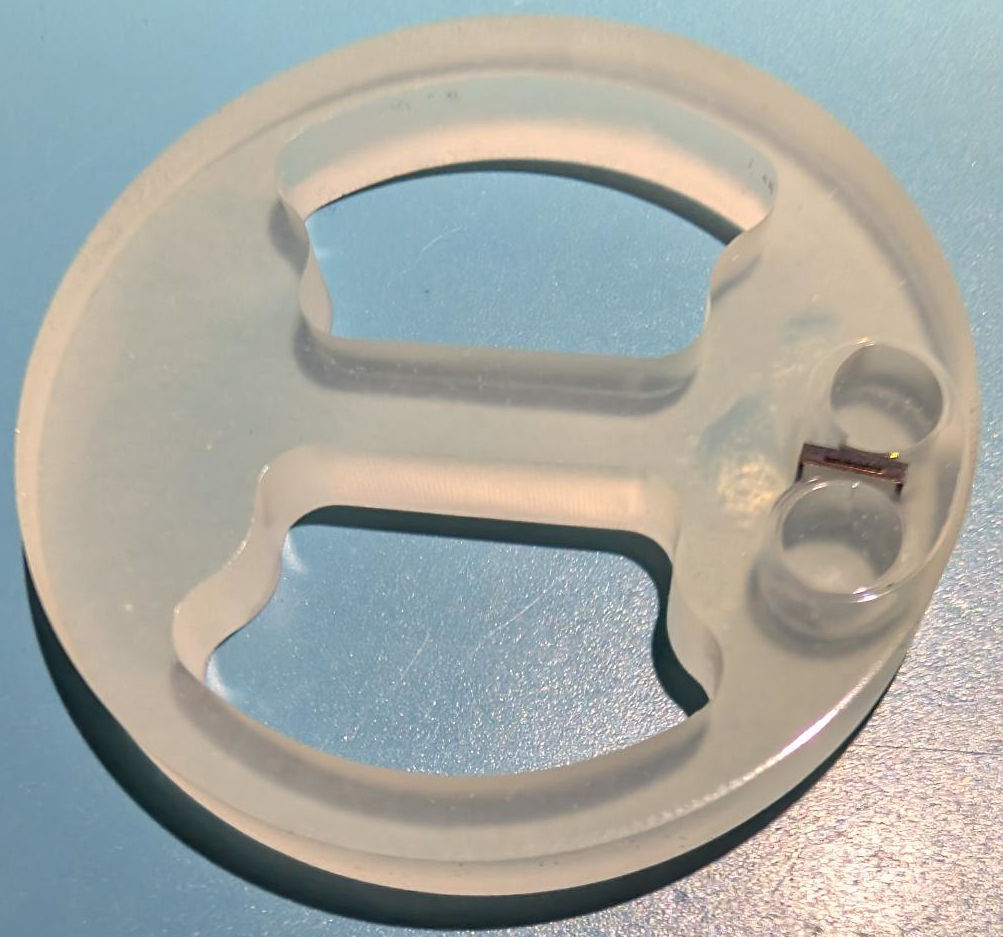
\includegraphics[width=12cm,keepaspectratio]{images/mount2.jpg}
\caption{Embedded package sample}
\label{mount}
\end{figure}

\begin{figure}[h]
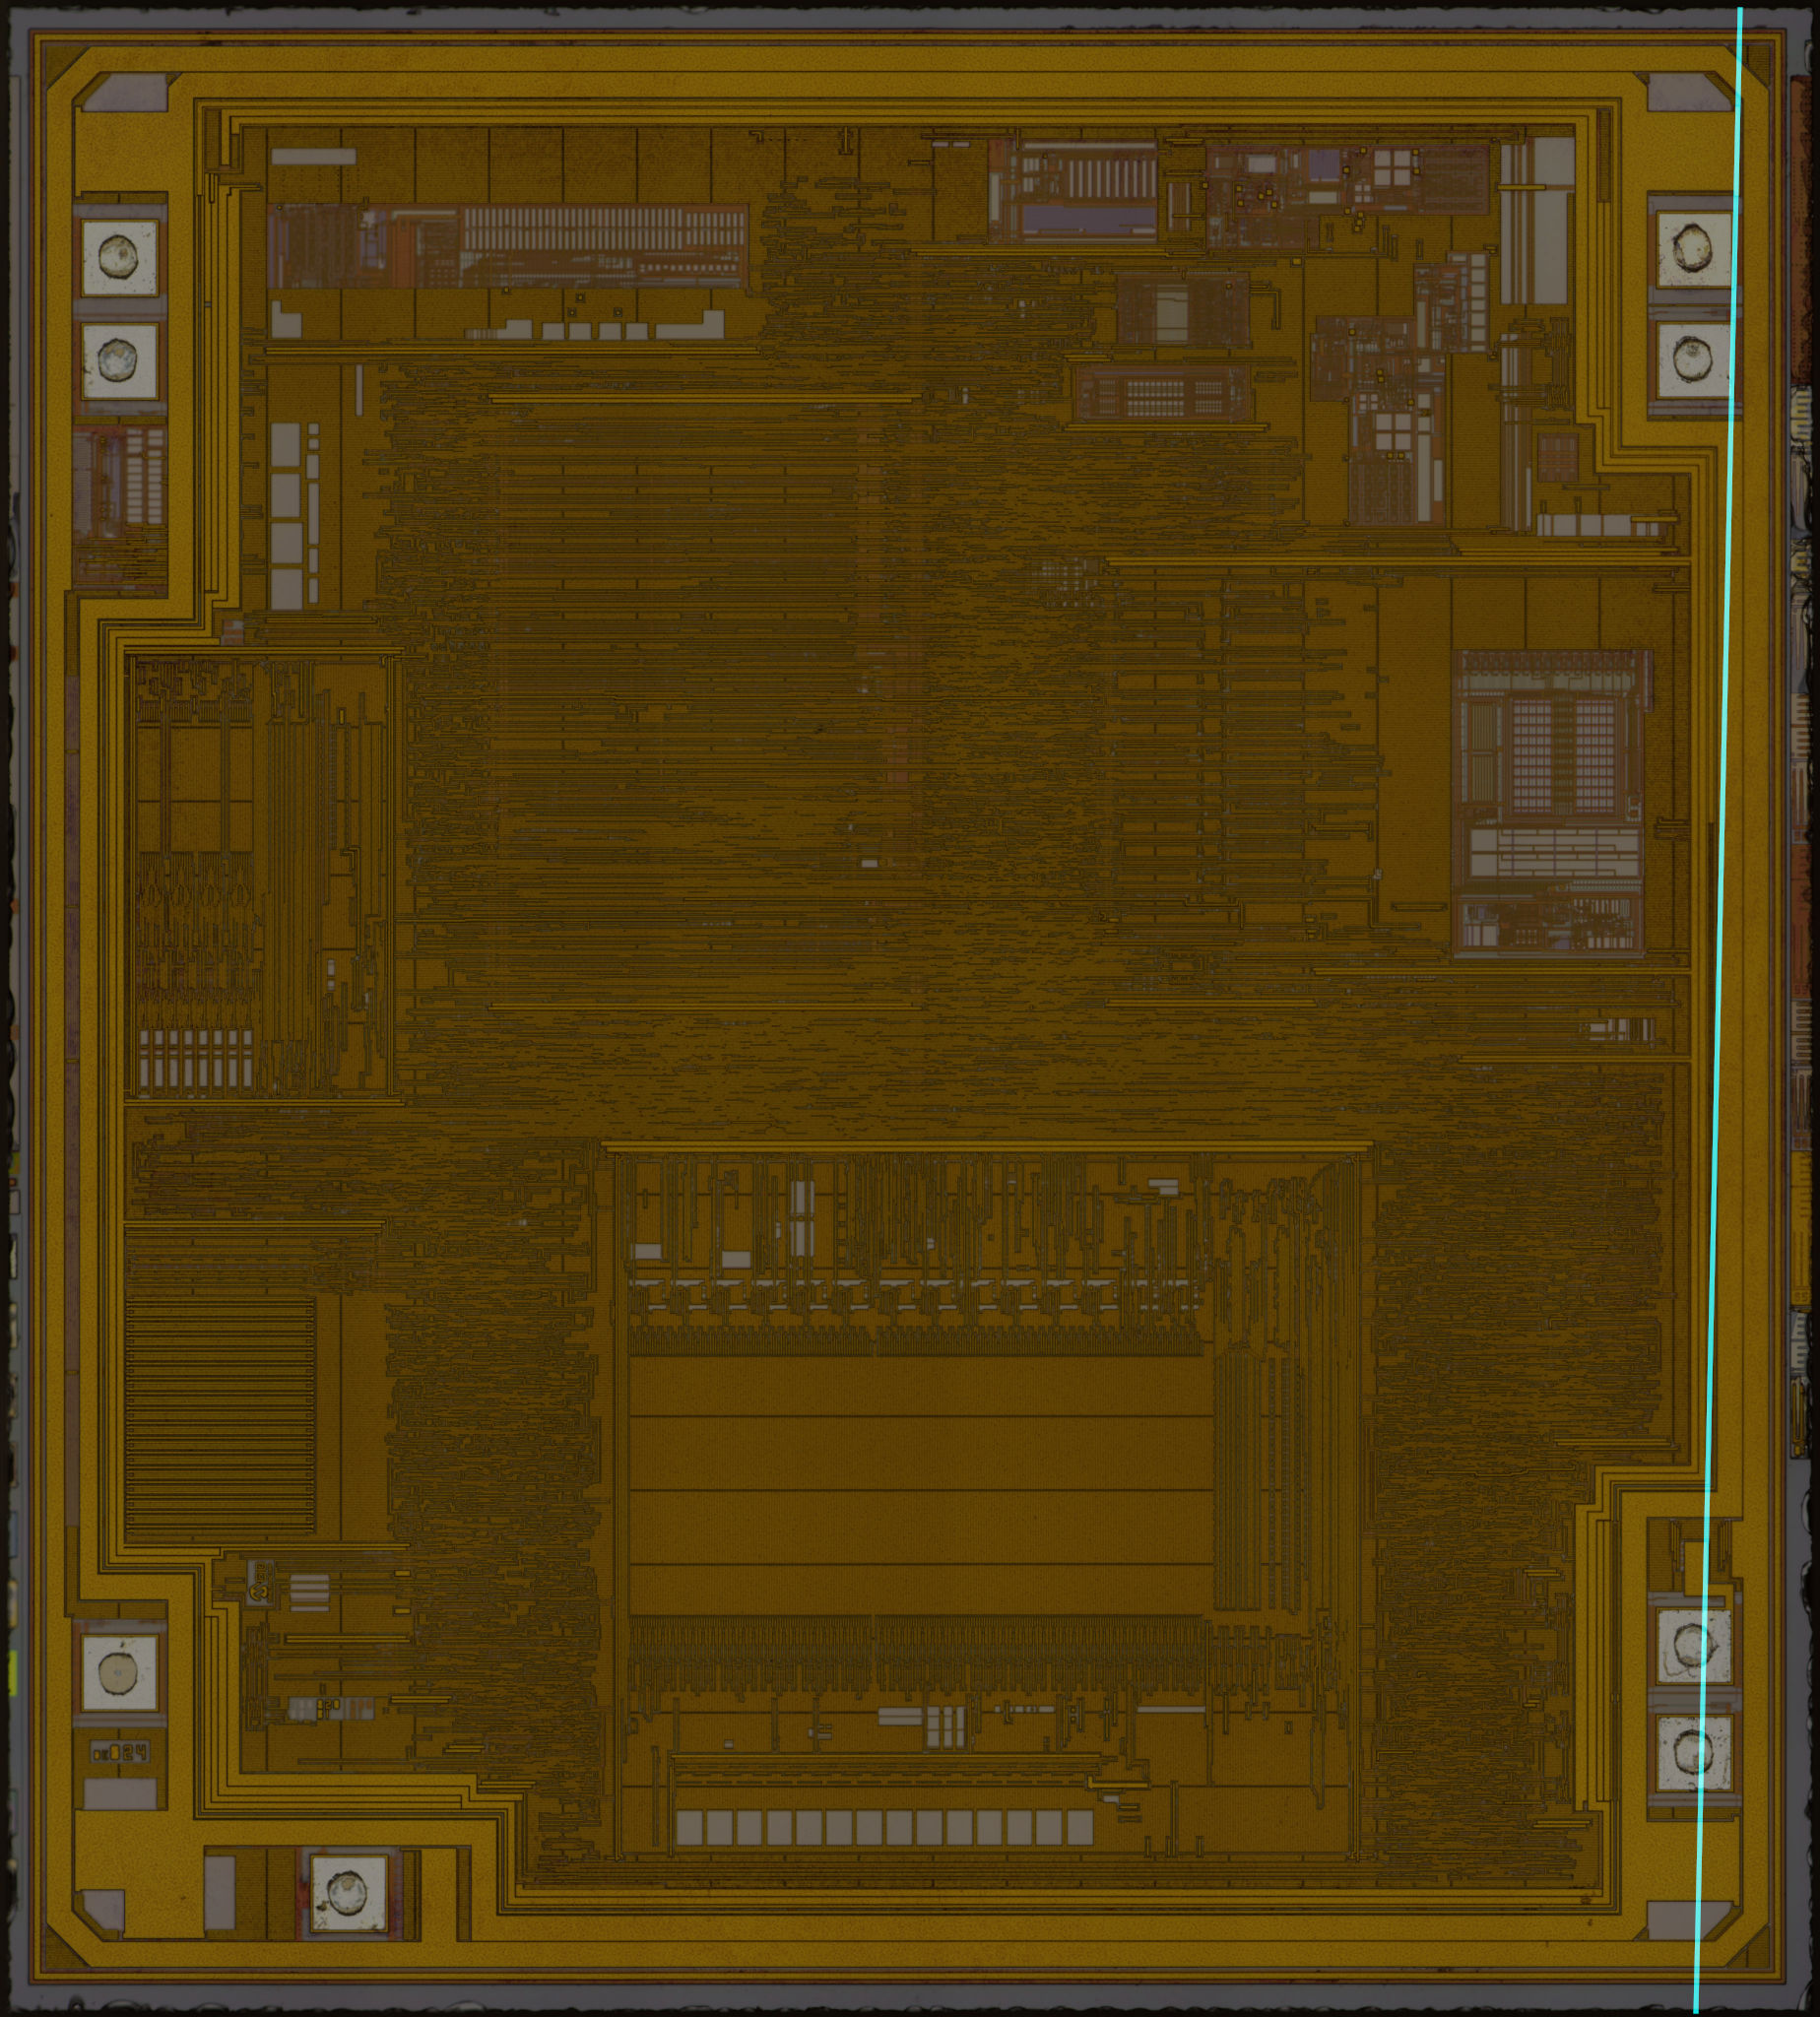
\includegraphics[width=12cm,keepaspectratio]{images/section-plane.jpg}
\caption{Approximate plane of the cross section. The camera position for the section is off the right side of the die, looking to the left.}
\label{section-plane}
\end{figure}

\begin{figure}[h]
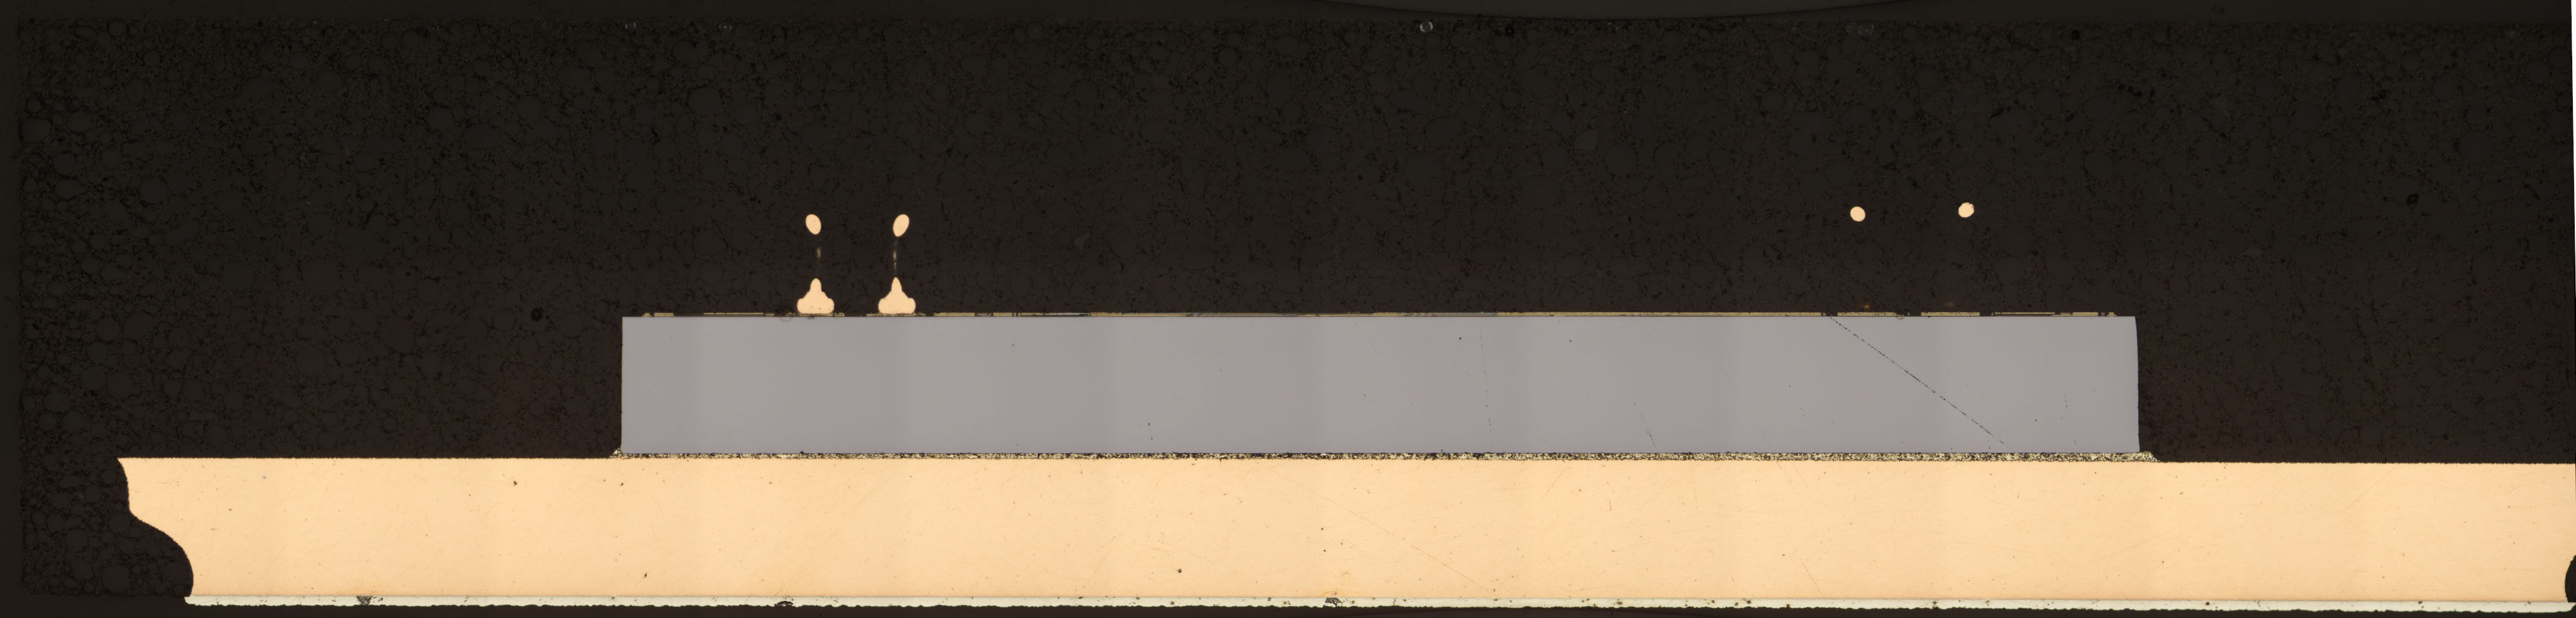
\includegraphics[width=12cm,keepaspectratio]{images/section.jpg}
\caption{Cross section of package. Pin 5/6 bond pads to the left, 7/8 to the right.}
\label{section}
\end{figure}

\FloatBarrier
\subsection{Partial Decapsulation}

\begin{figure}[h]
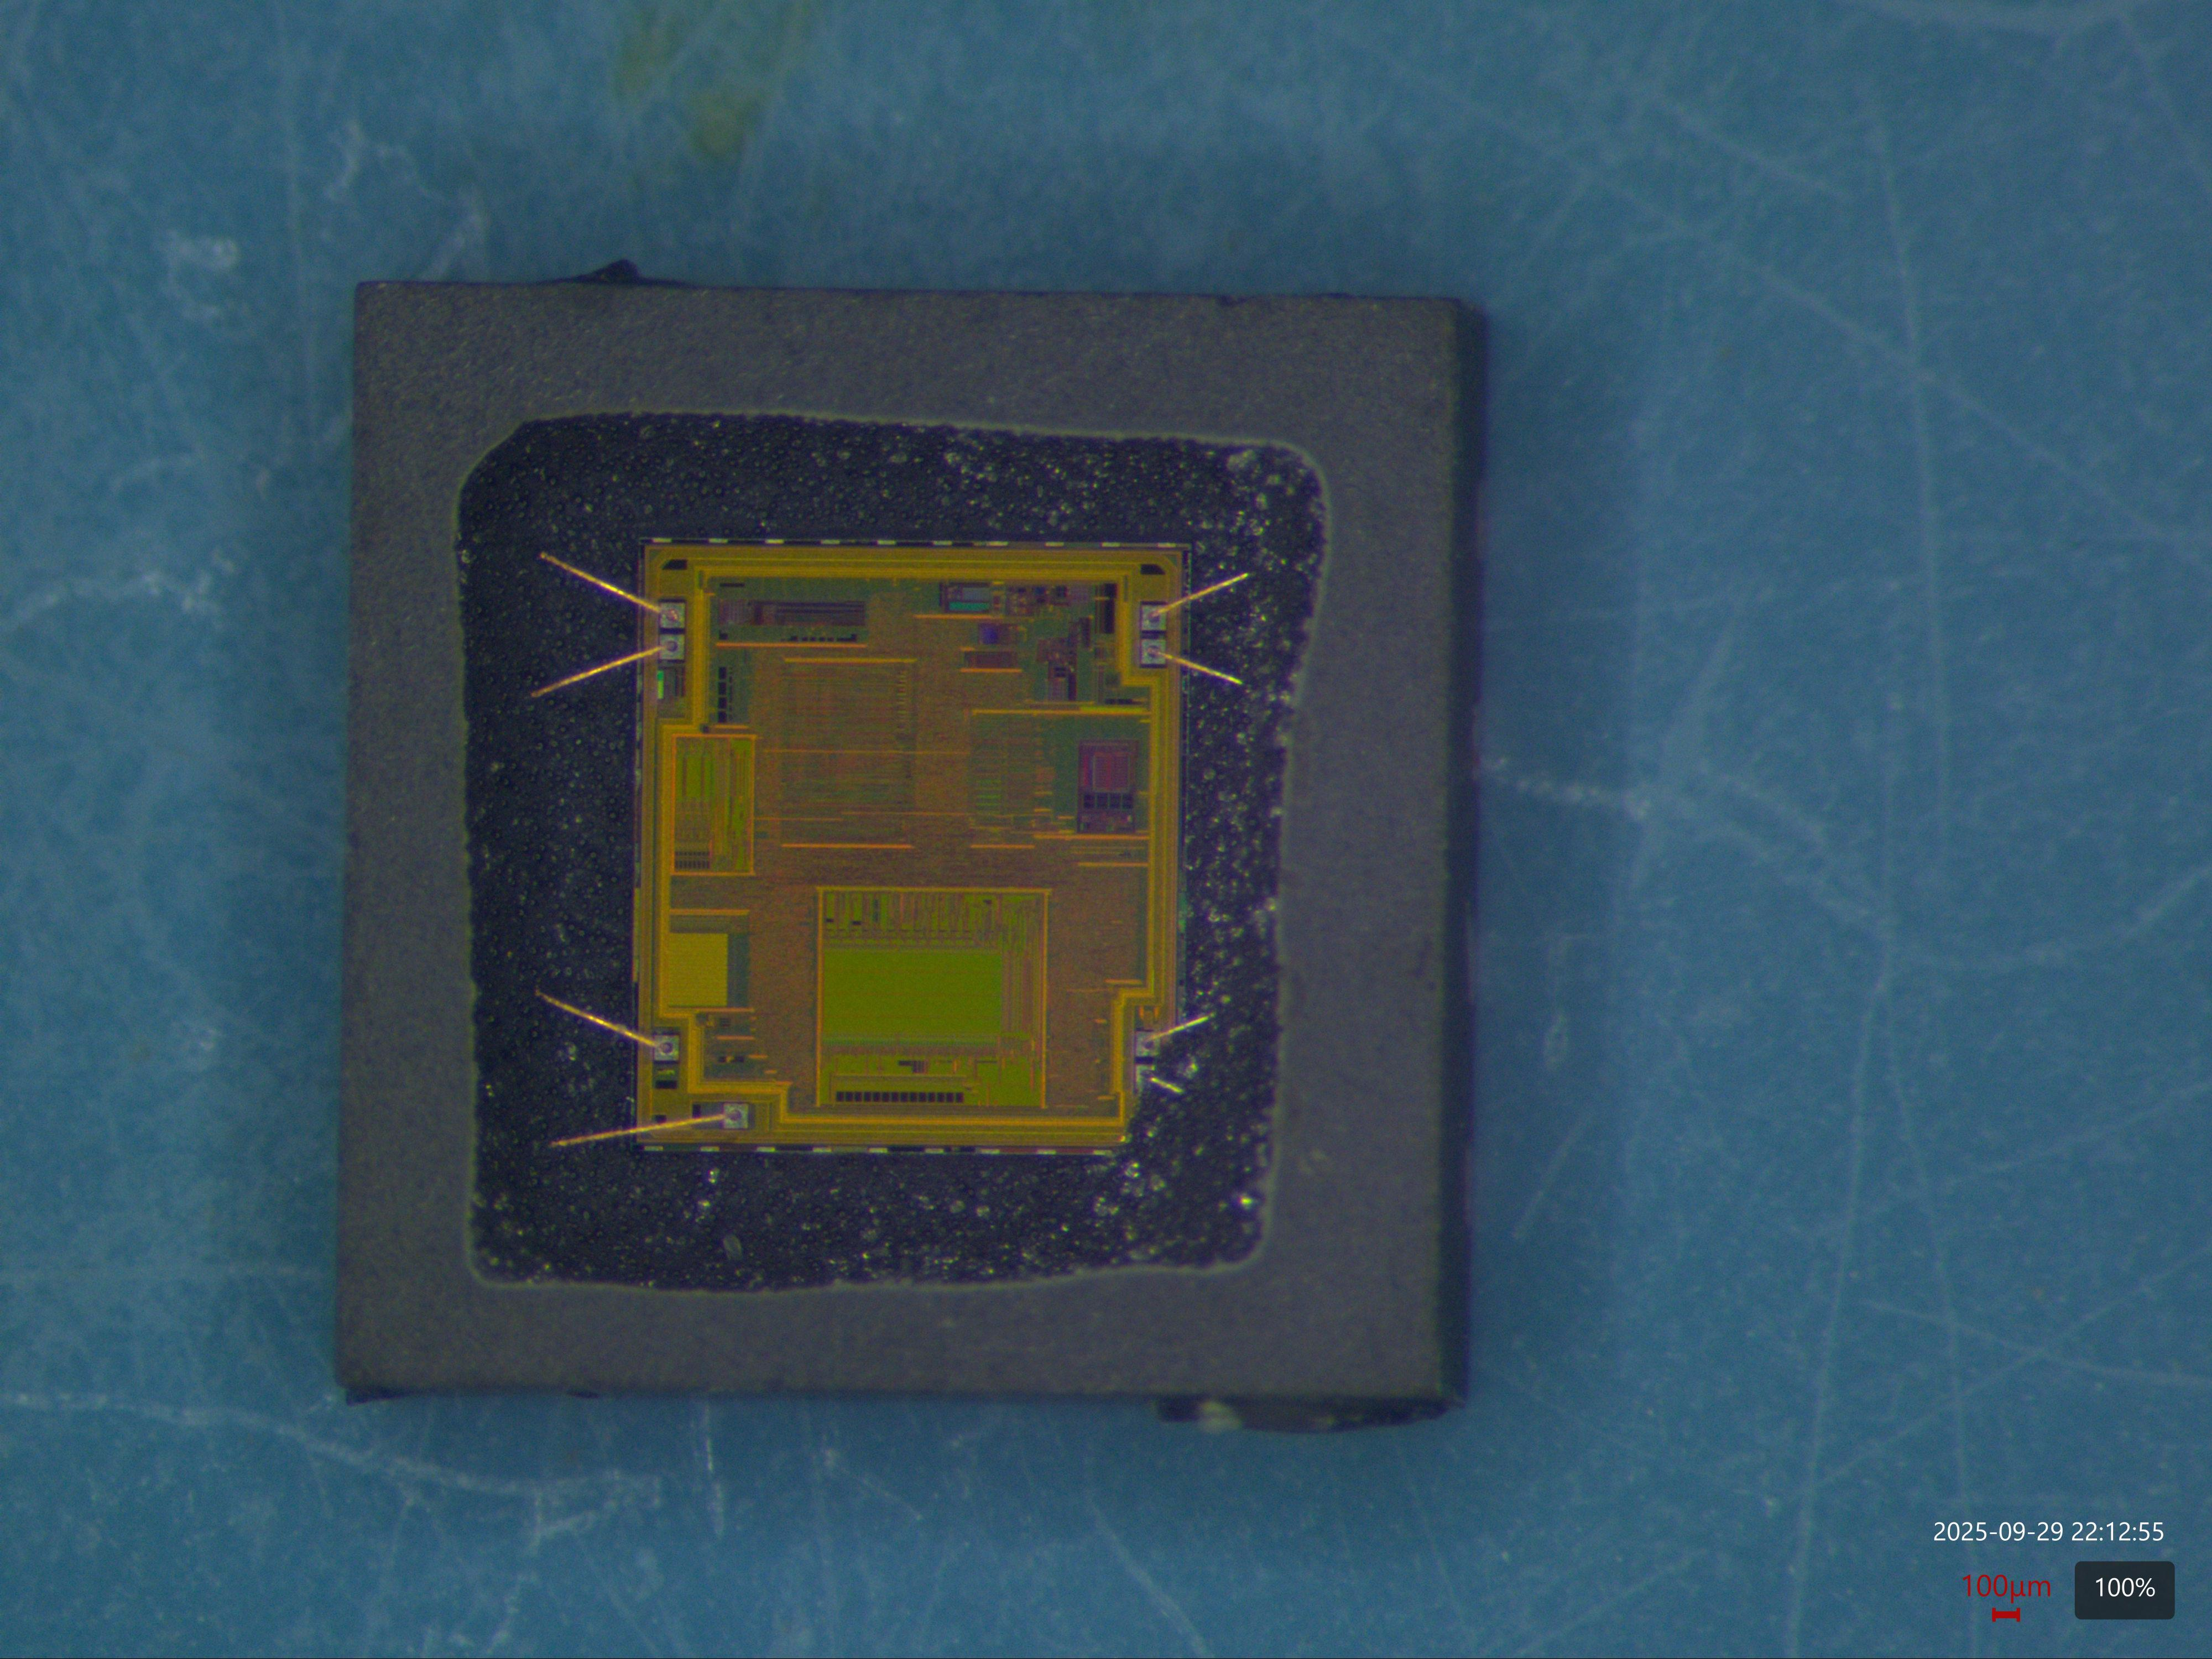
\includegraphics[width=12cm,keepaspectratio]{images/package-partial.jpg}
\caption{Package after partial decapsulation}
\label{package-partial}
\end{figure}

\begin{figure}[h]
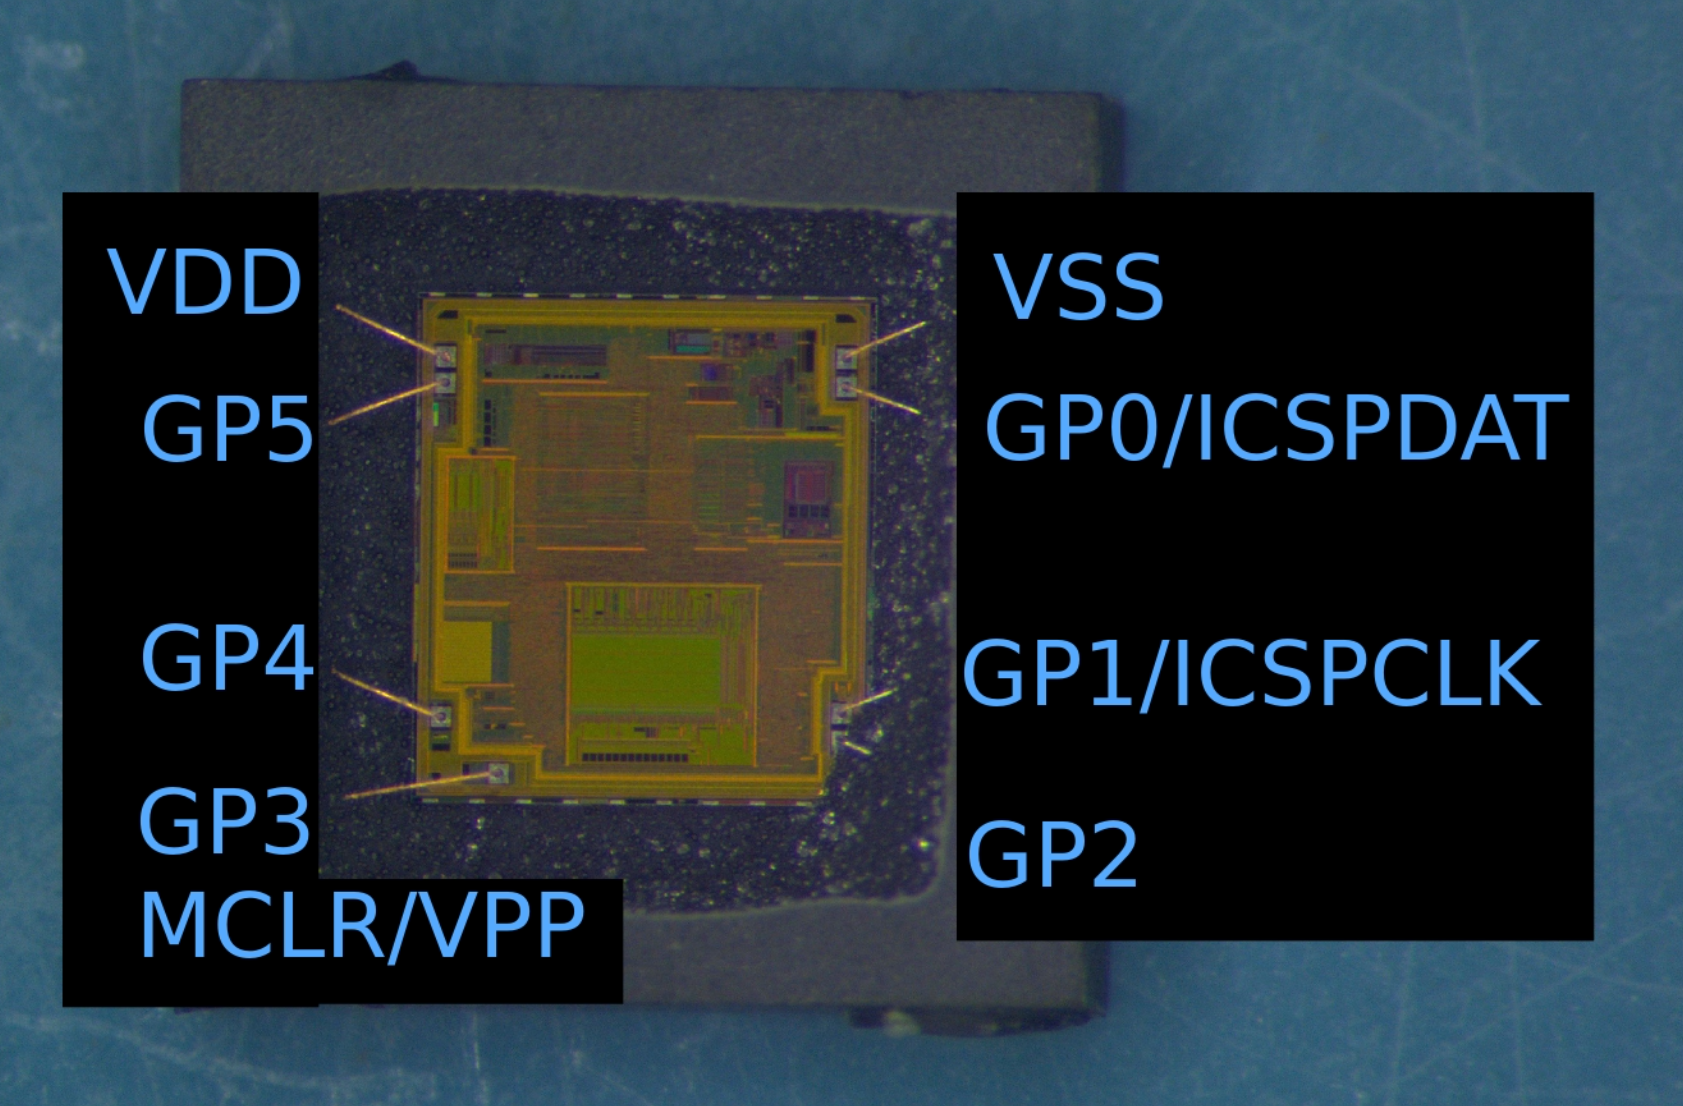
\includegraphics[width=12cm,keepaspectratio]{images/pins.png}
\caption{Package after partial decapsulation with pinout annotated}
\label{pinout-partial}
\end{figure}

\FloatBarrier
\pagebreak
\section{Process Analysis}

The die is made on Microchip's in-house 160K wafer
technology\footnote{\href{https://www.microchip.com/PCNWebAPI/api/pcn/DownloadPcnDocument?pcnId=10087&affectedcpns=pdf}{PCN
KSRA-19MSVX727}} at Fab 4 in Gresham, OR.

\pagebreak
\section{Device Floorplan Analysis}

\pagebreak
\section{SRAM}

\pagebreak
\section{EEPROM}

\pagebreak
\section{Flash}

\pagebreak
\section{Configuration Register}

\pagebreak
\section{CPU Core}

\pagebreak
\section{Conclusions}

\end{document}
